\documentclass{beamer}
% Setup for bibliography
\usepackage[
backend=biber,
style=numeric-comp,
]{biblatex}
\addbibresource{../../references.bib}

% Pretty self explanatory
% We sue this in title bits
\usepackage{datetime}

% Standard math packages / setup
\usepackage{amsmath} 
\usepackage{amsfonts}
\usepackage{amsthm}
\usepackage{amssymb} 
\usepackage{accents}
\usepackage{mathrsfs}
\usepackage{mathtools}

\usepackage{bm}

%\newtheorem{lemma}{Lemma}
%\newtheorem{theorem}{Theorem}
%\newtheorem{definition}{Definition}

% So we can import pngs
\usepackage{graphicx} 

% This gives us nice clickable links 
% https://www.overleaf.com/learn/latex/Hyperlinks#Styles_and_colours
\usepackage{hyperref}
\hypersetup{
    colorlinks=true,
    linkcolor=blue,
    citecolor=blue,
    filecolor=magenta,      
    urlcolor=cyan,
    pdftitle={Monte Carlo Methods (DRAFT)},
    pdfpagemode=FullScreen,
    }
\urlstyle{same}

% Allows us to define colors
% We use this in the next block, listings
\usepackage{color}
\definecolor{dkgreen}{rgb}{0,0.6,0}
\definecolor{gray}{rgb}{0.5,0.5,0.5}
\definecolor{mauve}{rgb}{0.58,0,0.82}

% Allows us to include 
\usepackage{listings}
\lstset{frame=tb,
  language={},
  aboveskip=3mm,
  belowskip=3mm,
  showstringspaces=false,
  columns=flexible,
  basicstyle={\small\ttfamily},
  numbers=none,
  numberstyle=\tiny\color{gray},
  keywordstyle=\color{blue},
  commentstyle=\color{dkgreen},
  stringstyle=\color{mauve},
  breaklines=true,
  breakatwhitespace=true,
  tabsize=4
}

% Adds bulletized outlines with outline environment
\usepackage{outlines}

% Tikz
\usepackage{tikz}

% Colors
\usepackage{xcolor}
\definecolor{uconnblue}{rgb}{0.08, 0.18, 0.28}
\definecolor{intactblue}{rgb}{0.13, 0.26, 0.45}
\definecolor{mastercamred}{rgb}{0.83, 0.01, 0.23}

% By default beamer slides are 4:3 , 128mm by 96mm

\logo{
\includegraphics[height=0.5cm]{../../assets/SBU_logos/horz_2clr_rgb_300ppi.png}}

\usetheme{CambridgeUS}

\AtBeginSection[]
{
  \begin{frame}
    \frametitle{Table of Contents}
    \tableofcontents[currentsection]
  \end{frame}
}

% \shadowimage[width=8cm]{image}
%
% Provides a drop-shadow to images
%
% From
% https://tex.stackexchange.com/questions/81842/creating-a-drop-shadow-with-guassian-blur 
\usetikzlibrary{shadows,calc}

% code adapted from https://tex.stackexchange.com/a/11483/3954

% some parameters for customization
\def\shadowshift{3pt,-3pt}
\def\shadowradius{6pt}

\colorlet{innercolor}{black!60}
\colorlet{outercolor}{gray!05}

% this draws a shadow under a rectangle node
\newcommand\drawshadow[1]{
    \begin{pgfonlayer}{shadow}
        \shade[outercolor,inner color=innercolor,outer color=outercolor] ($(#1.south west)+(\shadowshift)+(\shadowradius/2,\shadowradius/2)$) circle (\shadowradius);
        \shade[outercolor,inner color=innercolor,outer color=outercolor] ($(#1.north west)+(\shadowshift)+(\shadowradius/2,-\shadowradius/2)$) circle (\shadowradius);
        \shade[outercolor,inner color=innercolor,outer color=outercolor] ($(#1.south east)+(\shadowshift)+(-\shadowradius/2,\shadowradius/2)$) circle (\shadowradius);
        \shade[outercolor,inner color=innercolor,outer color=outercolor] ($(#1.north east)+(\shadowshift)+(-\shadowradius/2,-\shadowradius/2)$) circle (\shadowradius);
        \shade[top color=innercolor,bottom color=outercolor] ($(#1.south west)+(\shadowshift)+(\shadowradius/2,-\shadowradius/2)$) rectangle ($(#1.south east)+(\shadowshift)+(-\shadowradius/2,\shadowradius/2)$);
        \shade[left color=innercolor,right color=outercolor] ($(#1.south east)+(\shadowshift)+(-\shadowradius/2,\shadowradius/2)$) rectangle ($(#1.north east)+(\shadowshift)+(\shadowradius/2,-\shadowradius/2)$);
        \shade[bottom color=innercolor,top color=outercolor] ($(#1.north west)+(\shadowshift)+(\shadowradius/2,-\shadowradius/2)$) rectangle ($(#1.north east)+(\shadowshift)+(-\shadowradius/2,\shadowradius/2)$);
        \shade[outercolor,right color=innercolor,left color=outercolor] ($(#1.south west)+(\shadowshift)+(-\shadowradius/2,\shadowradius/2)$) rectangle ($(#1.north west)+(\shadowshift)+(\shadowradius/2,-\shadowradius/2)$);
        \filldraw ($(#1.south west)+(\shadowshift)+(\shadowradius/2,\shadowradius/2)$) rectangle ($(#1.north east)+(\shadowshift)-(\shadowradius/2,\shadowradius/2)$);
    \end{pgfonlayer}
}

% create a shadow layer, so that we don't need to worry about overdrawing other things
\pgfdeclarelayer{shadow} 
\pgfsetlayers{shadow,main}


\newcommand\shadowimage[2][]{%
\begin{tikzpicture}
\node[anchor=south west,inner sep=0] (image) at (0,0) {\includegraphics[#1]{#2}};
\drawshadow{image}
\end{tikzpicture}}



% Remove drop shadow by title
% https://tex.stackexchange.com/questions/3139/beamer-how-to-remove-shadow-under-the-title-on-a-given-frame
\setbeamertemplate{title page}[default][colsep=-4bp,rounded=true]

%gets rid of footer
%will override 'frame number' instruction above
%comment out to revert to previous/default definitions
\setbeamertemplate{footline}{}

%gets rid of bottom navigation symbols
\setbeamertemplate{navigation symbols}{}


\setbeamerfont*{frametitle}{family=\rmfamily, parent=structure}

%Information to be included in the title page:
\title{Quake: Adaptive Indexing for Vector Search}
\author{
  Jason Mohoney \inst{1} 
  \and Devesh Sarda \inst{1}
  \and Mengze Tang \inst{1}
  \and Shihabur Rahman Chowdhury \inst{2}
  \and Anil Pacaci \inst{2}
  \and Ihab F. Ilyas \inst{3} 
  \and Theodoros Rekatsinas \inst{2}
  \and Shivaram Venkatarama \inst{1}
}
\institute[shortinst]{
  \inst{1} University of Wisconsin–Madison 
  \and \inst{2} Apple
  \and \inst{3} University of Waterloo 
}

\date{OSDI 2025}

\begin{document}
\fontfamily{cmr}\selectfont

\frame{\titlepage \blfootnote{Presented by Russell Bentley}}

\placelogofalse
\begin{frame}{Vector Search: Algorithm Problem}
\begin{columns}
\column{0.48\linewidth}
\begin{outline}
  \1 Search $N$ vectors in $D$ dimensions 
  \2 $k$-nearest Neighbor (KNN) 
  \2 Approximate nearest neighbor (ANN)
\end{outline}

\vspace{0.2cm}

$$
\text{Recall (Accuracy)} = \frac{G \cap R}{k}
$$
Where
\begin{align*}
  G &= \text{Ground Truth} \\
  R &= \text{Results}
\end{align*}

\column{0.48\linewidth}
\begin{center}
\centering
% [trim={left bottom right top},clip]
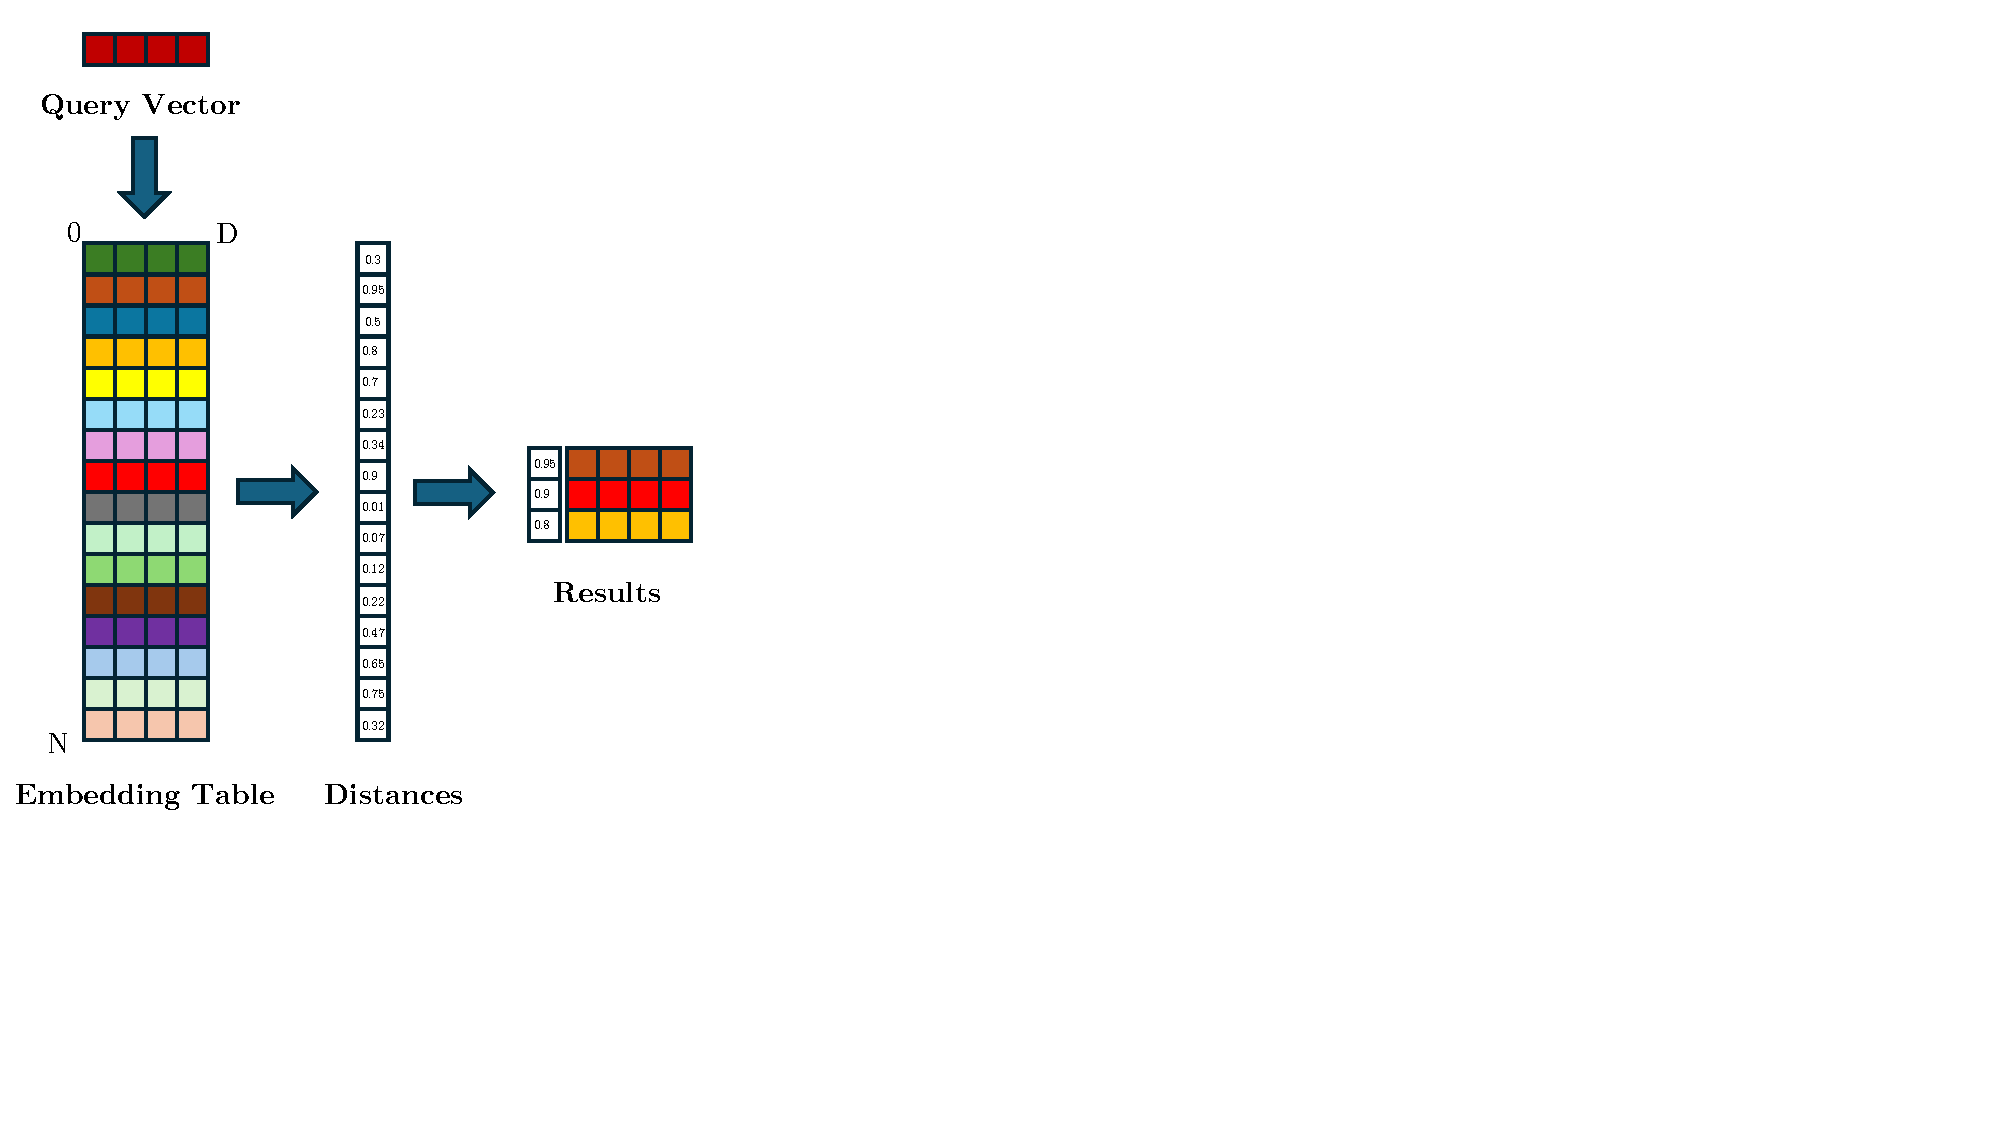
\includegraphics[width=5.0cm, page=1, trim={0 5cm 22cm 0cm},clip]{assets/vec_db_figs.pdf}

\end{center}
\end{columns}
\end{frame}
\placelogotrue



\placelogofalse
\begin{frame}{Vector Search: Applications}
\begin{columns}
  \column{0.48\linewidth}
  \begin{outline}
  \1 \textbf{Machine Learning}
  \1 Retrieval Augmented Generation
  \1 Recomendations Systems
  \1 Similarity Search
\end{outline}
  \column{0.48\linewidth}
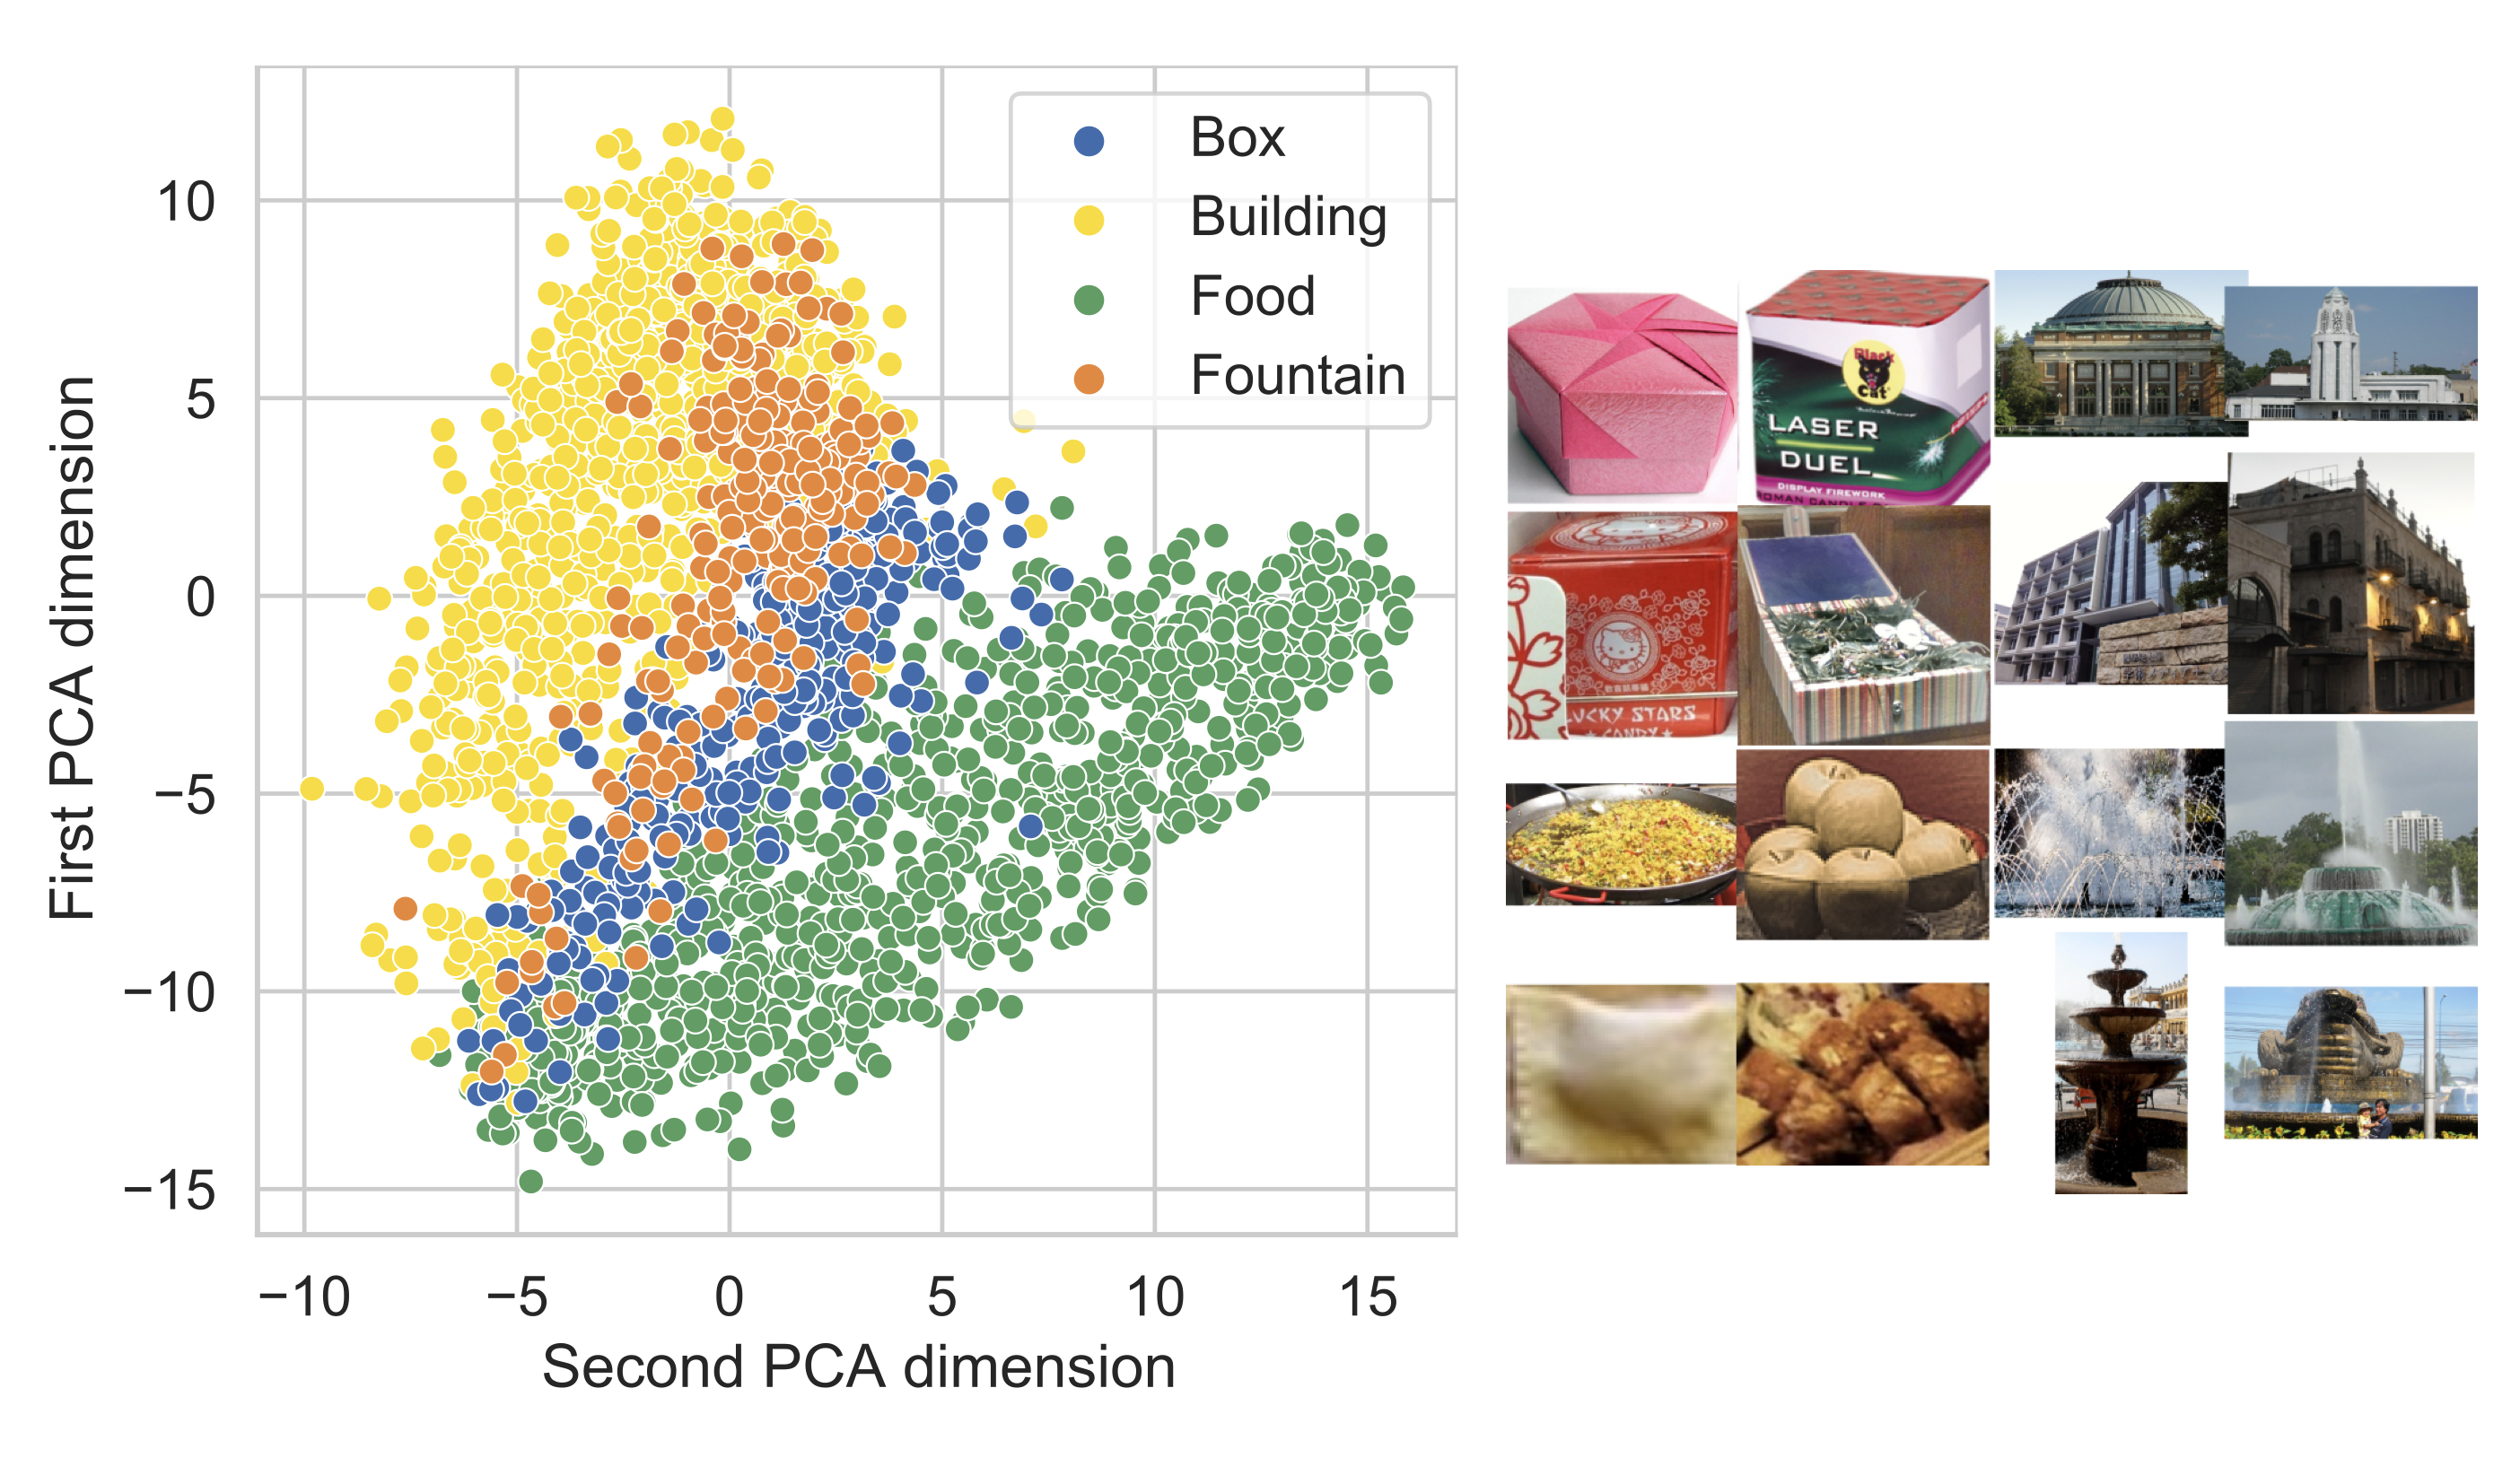
\includegraphics[width=5.0cm]{assets/image_vec.png}

{\tiny From \href{https://github.com/intel/ScalableVectorSearch}{ScalableVectorSearch}}

\end{columns}
\begin{center}
\centering
%\shadowimage[width=2.5cm]{example_1.png}

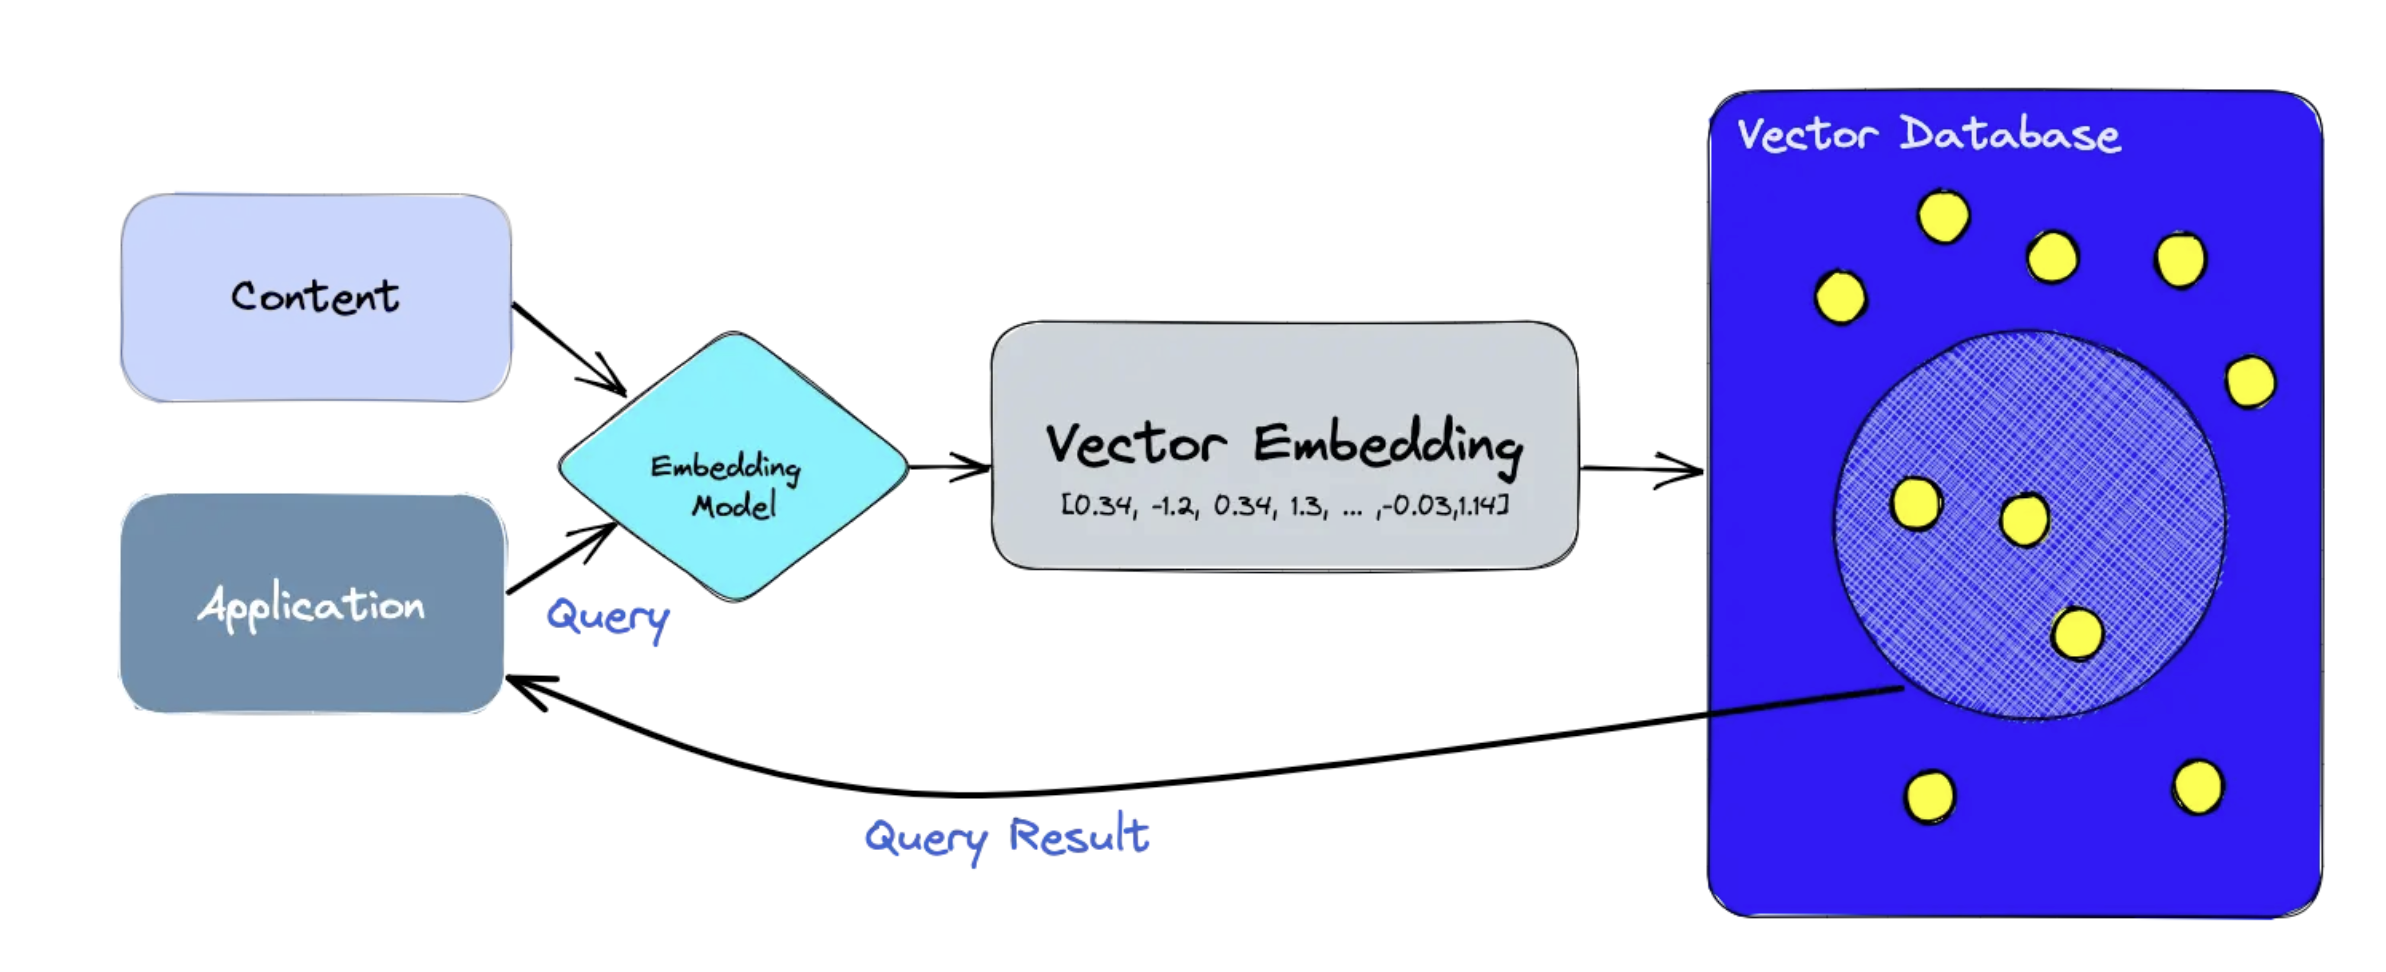
\includegraphics[width=8.5cm]{assets/vec_workflow.png}

{\tiny From \href{https://pages.cs.wisc.edu/~shivaram/cs744-sp25-slides/cs744-lyticdb-v.pdf}{Shivaram's CS744 Slides}}

\end{center}
\end{frame}
\placelogotrue




%\placelogofalse
\begin{frame}{Vector Search: Production Workloads}
\begin{columns}
\column{0.58\linewidth}
\centering
\begin{outline}
  \1 SOTA focusses on Static / semi static data
  \1 Production workloads are dynamic 
  \1 Data can be inserted, removed, edited
  \1 Require dynamic Indexing strategies
  \1 Metrics that matter:
  \2 Recall
  \2 Latency
\end{outline}

\column{0.38\linewidth}
\begin{center}
\centering
% [trim={left bottom right top},clip]
\includegraphics[width=4.5cm, page=4, trim={0 9cm 22cm 0cm},clip]{assets/vec_db_figs.pdf}

\end{center}
\end{columns}

\end{frame}
%\placelogotrue





\placelogofalse
\begin{frame}{Vector Search: Graph Indexing}
\begin{columns}
\column{0.48\linewidth}
\centering
\begin{outline}
  \1 Proximity graph
  \2 Node for each vector
  \2 Edge for (approx) neighbors 
  \1 Query is a graph traversal 
\end{outline}

\column{0.48\linewidth}
\begin{outline}
  \1 For static data:
  \2 High recall!
  \2 Low latency!
  \1 For dynamic data:
  \2 Expensive to initialize
  \2 Expensive to update 
\end{outline}
\end{columns}

\begin{center}
\centering

% [trim={left bottom right top},clip]
\includegraphics[width=8.5cm, page=3, trim={0 9cm 14cm 0cm},clip]{assets/vec_db_figs.pdf}

\end{center}
\end{frame}
\placelogotrue


\placelogofalse
\begin{frame}{Vector Search: Partioned Index}
\begin{columns}
\column{0.48\linewidth}
\centering
\begin{outline}
  \1 Partition into clusters
  \2 $k$-means or other method
  \1 Scan relevant clusters
  \2 Requires tuning (nprobe)
  \1 Easy to update
  \1 SOTA has latency issues
  \1 Imbalanced partitions
\end{outline}

\column{0.48\linewidth}
\begin{center}
\centering
% [trim={left bottom right top},clip]
\includegraphics[width=4.0cm, page=2, trim={0 7.5cm 21cm 0cm},clip]{assets/vec_db_figs.pdf}

\vspace{0.3cm}

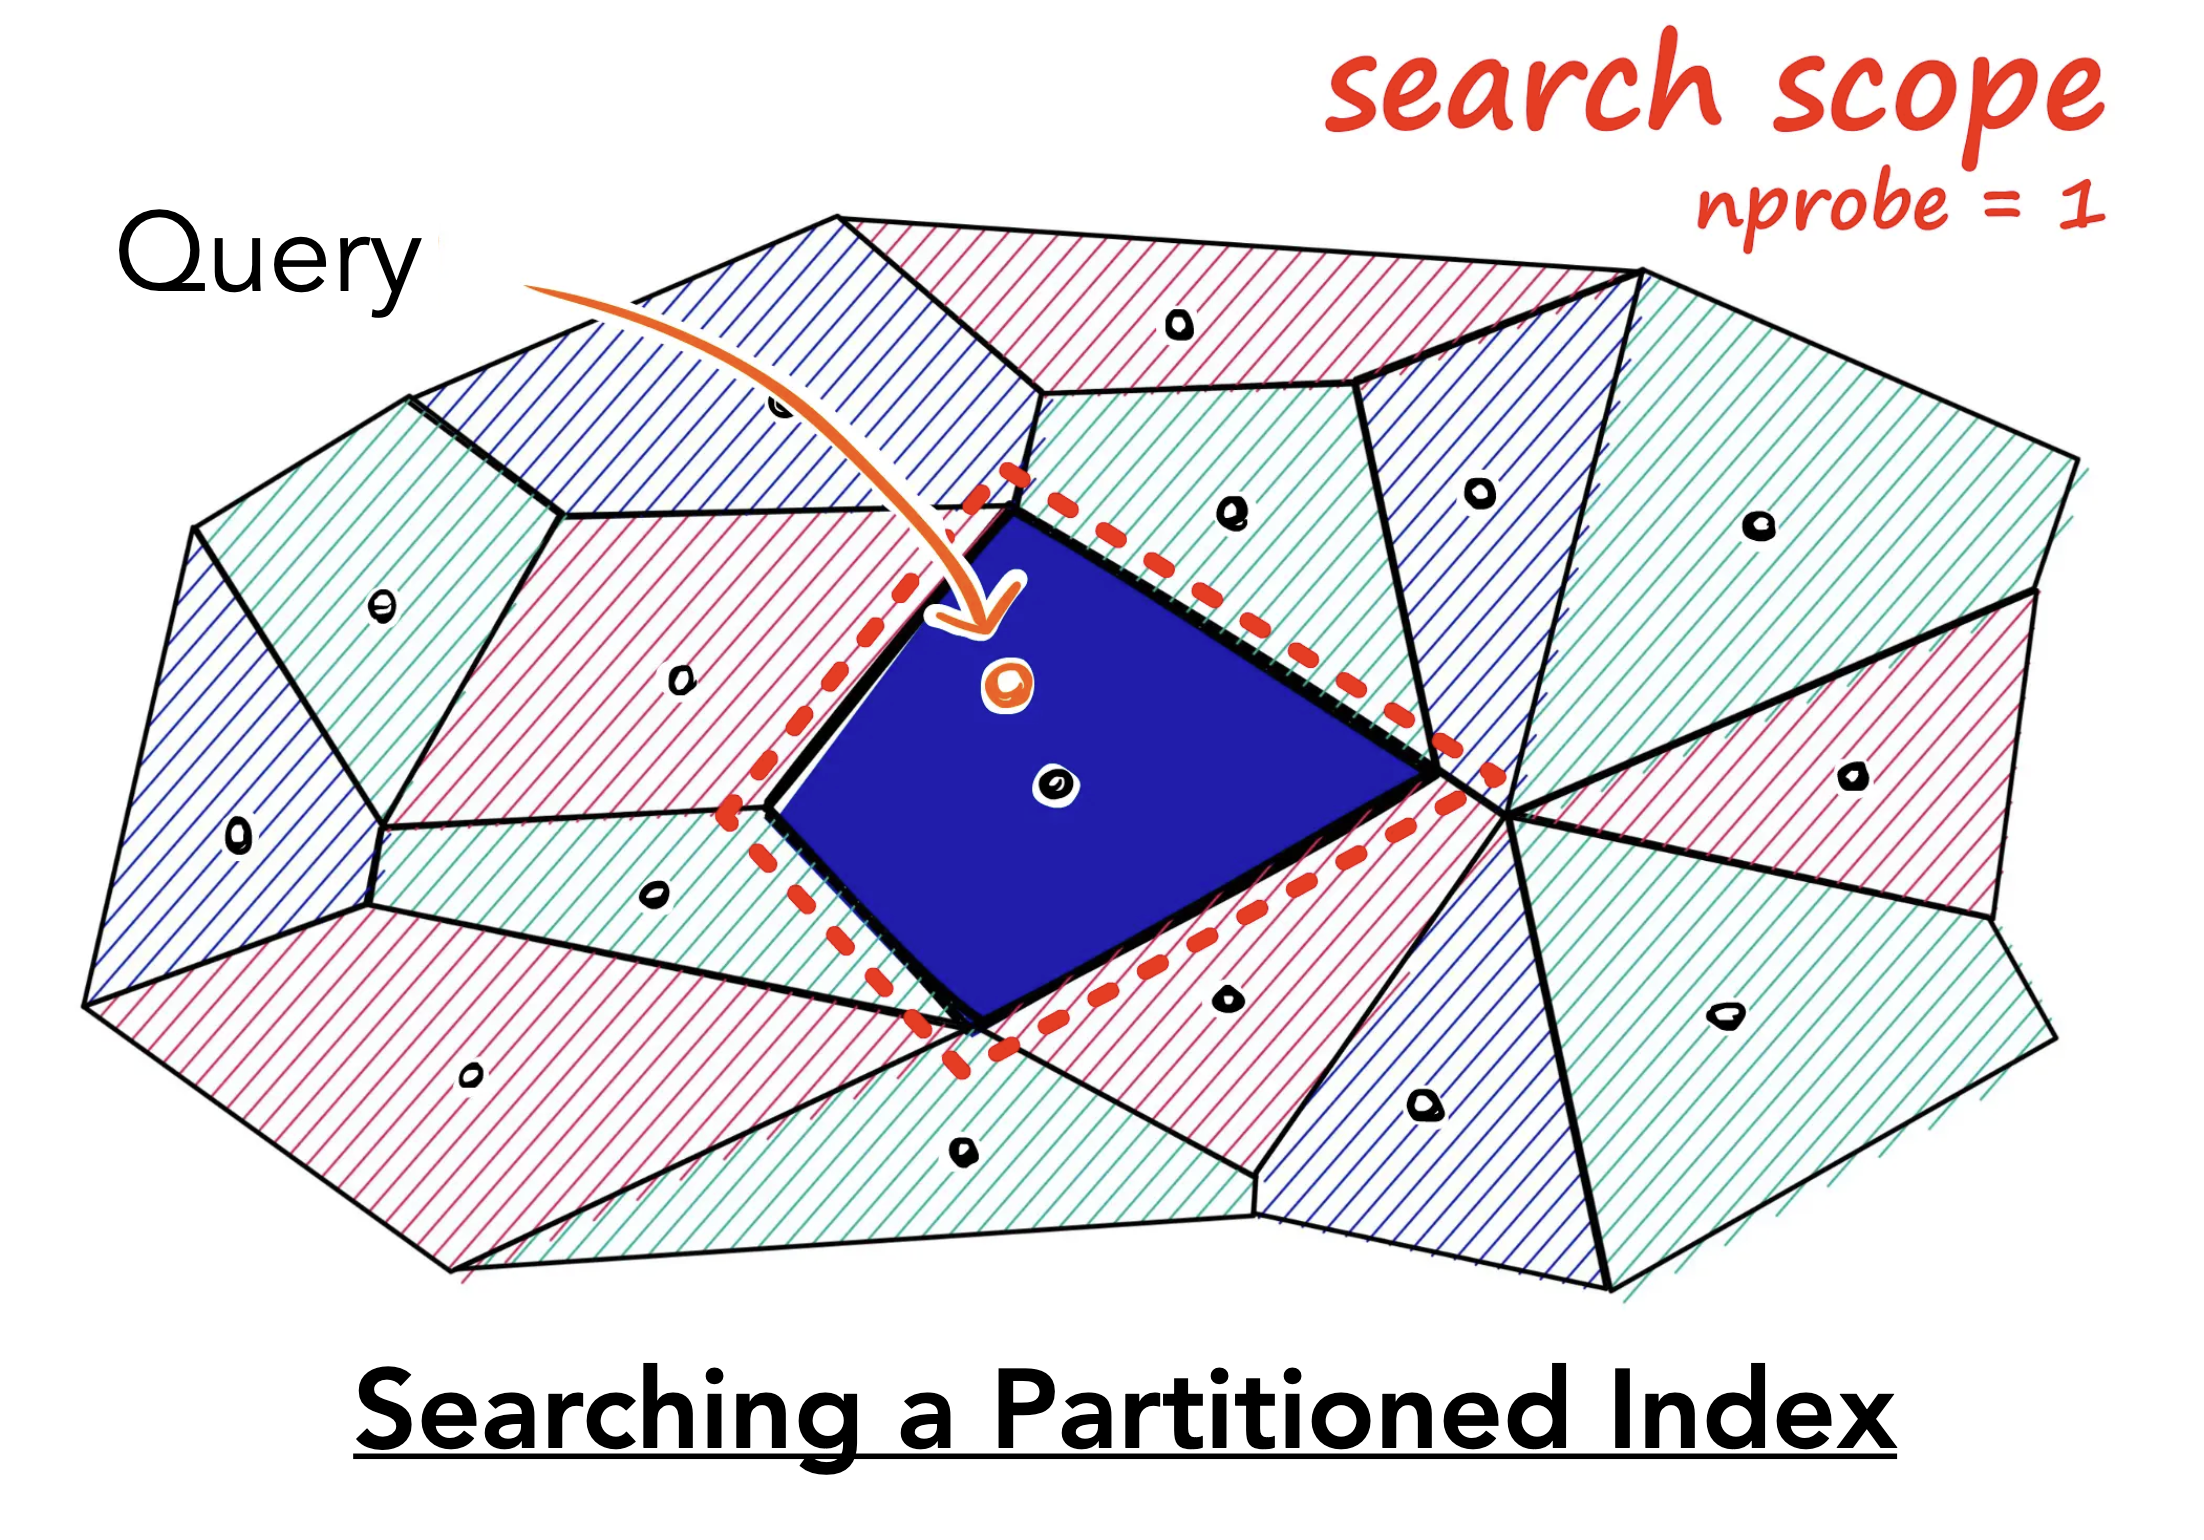
\includegraphics[width=4.5cm]{assets/partition_fig.png}

{\tiny From \href{https://pages.cs.wisc.edu/~shivaram/cs744-sp25-slides/cs744-analyticdb-v.pdf}{Shivaram's CS744 Slides}}

\end{center}
\end{columns}
\end{frame}
\placelogotrue


\placelogofalse
\begin{frame}{Vector Search: Challenges}
\begin{columns}
\column{0.38\linewidth}
\centering
\begin{outline}
  \1 Memory Bound
  \1 Skewed Reads
  \1 Dynamic Data 
  \1 Skewed Writes
  \1 Recall
  \1 Latency 
\end{outline}

\column{0.58\linewidth}
\begin{center}
\centering
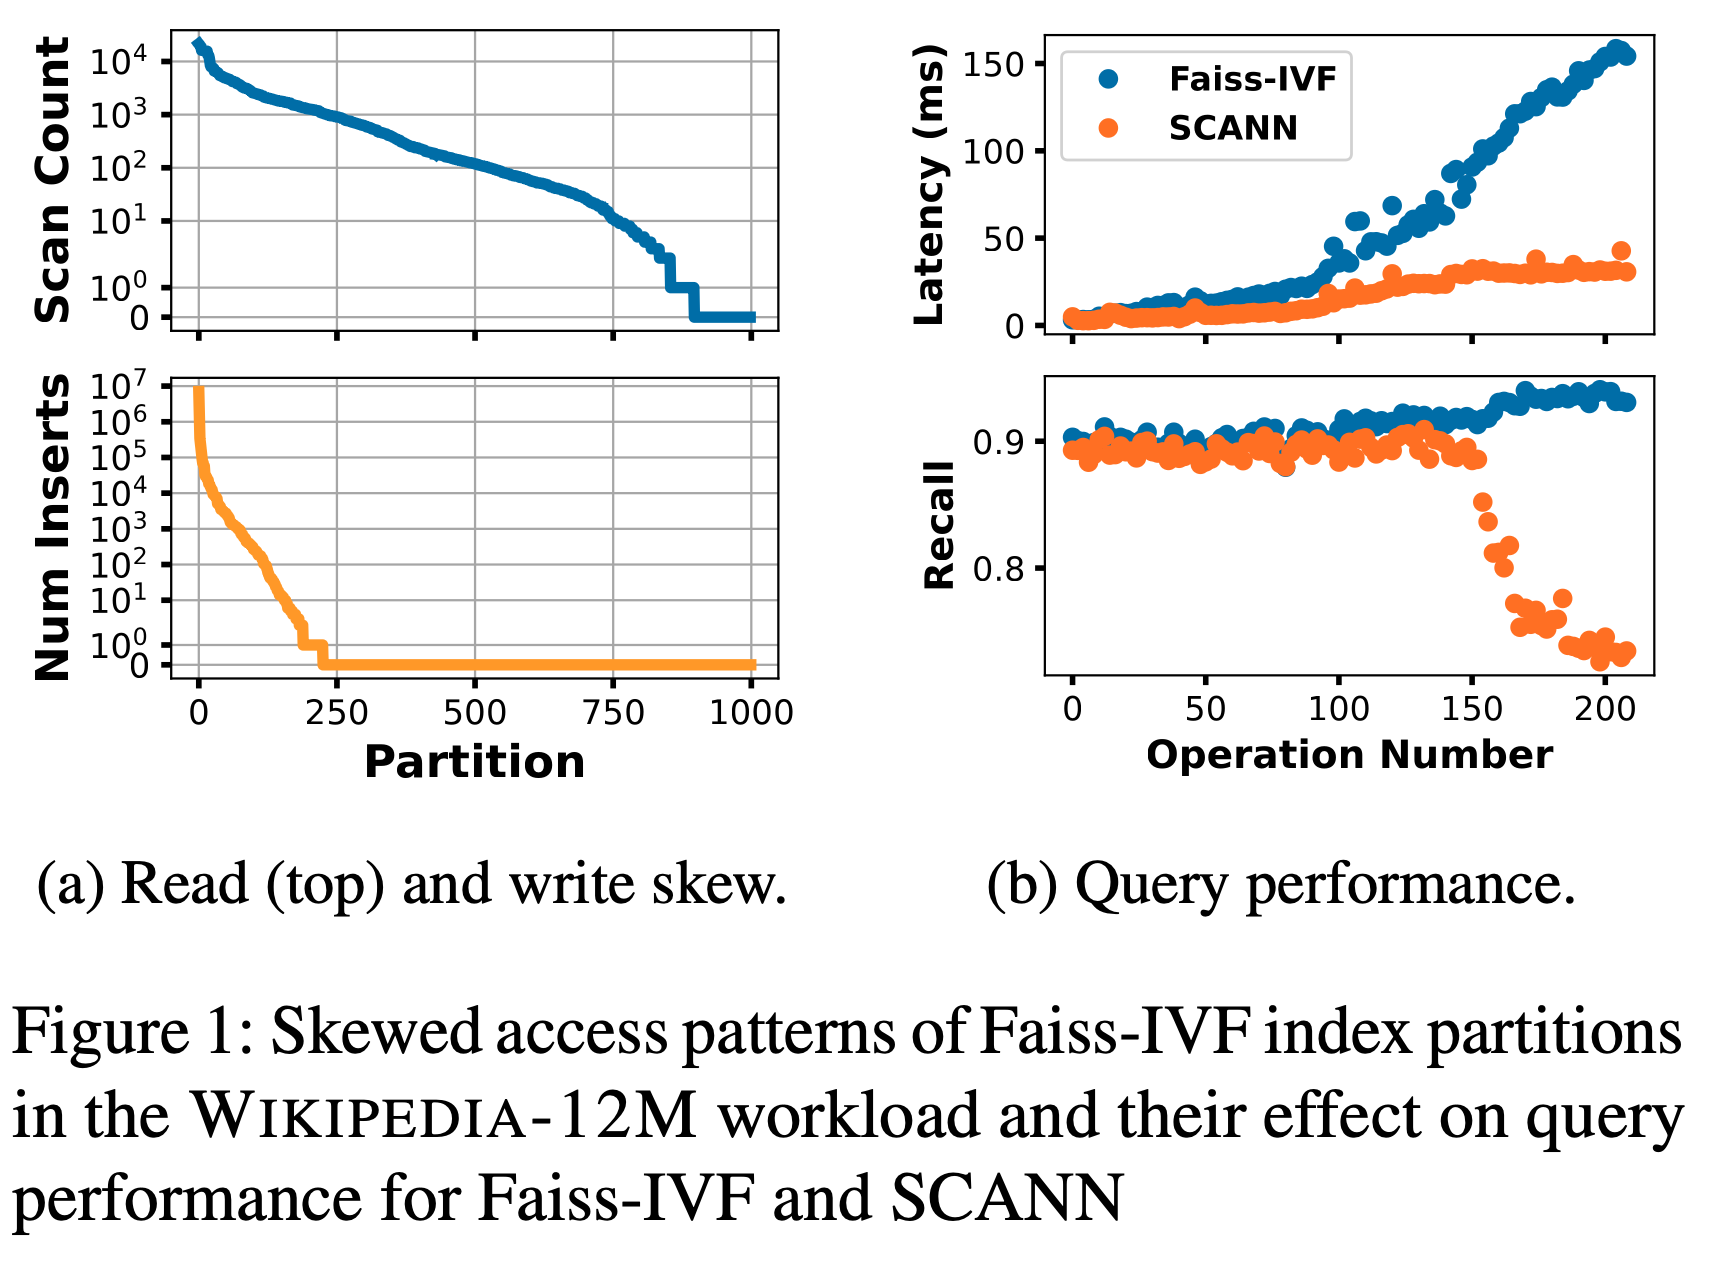
\includegraphics[width=7cm]{assets/fig_1_t2.png}

\end{center}
\end{columns}
\end{frame}
\placelogotrue





\section{Quake}

%\placelogofalse
\begin{frame}{Quake Introduction}
``In this work, we study the problem of minimizing query latency to meet a fixed recall target for dynamic vector search.''
\begin{columns}
\column{0.58\linewidth}
\centering
\begin{outline}
  \1 Adaptive Hierarchical partioning
  \1 Adaptive Partition Scanning
  \1 NUMA aware parallelism
\end{outline}

\column{0.38\linewidth}
\begin{center}
\centering
%\shadowimage[width=2.5cm]{example_1.png}

\end{center}
\end{columns}
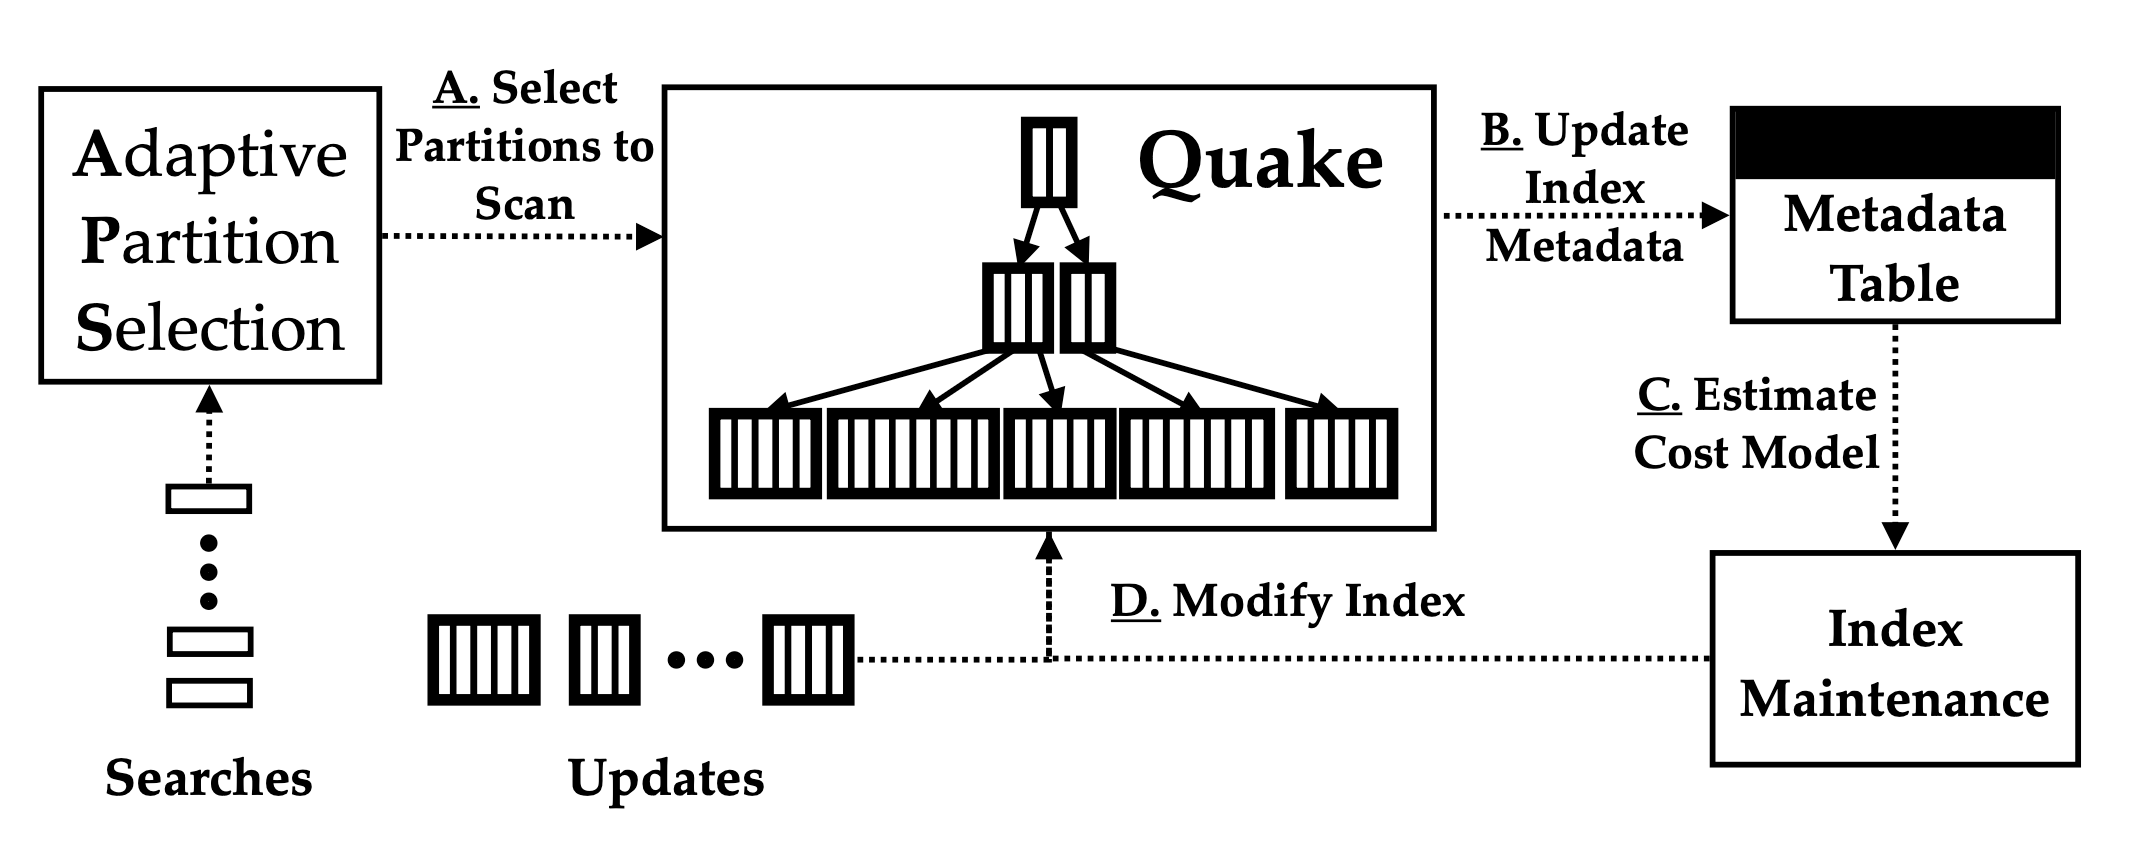
\includegraphics[width=2.5cm]{assets/quake_arch.png}
\end{frame}
%\placelogotrue


\subsection{Cost-Driven Maintenance}

%\placelogofalse
\begin{frame}{Const-Driven Maintenance}
Use a cost-model for query latency to determine which partitions to split / merge.
\begin{columns}
\column{0.48\linewidth}
\begin{align*}
  C &= \sum_{i}C_i \ \text{Total cost (latency)}\\
  C_i &= O_c + A_i \lambda(s_i) \ \text{Per-partition cost}\\
\end{align*}
\column{0.48\linewidth}
\begin{align*}
  A_i & \ \text{Access frequency of partition }i \\
  s_i & \ \text{Since of partition }i \\
  \lambda(s_i) & \ \text{Latency to scan partition } i \\
O_c & \ \text{Latency to scan centroid}
\end{align*}
\end{columns}
Estimate the change in cost of a split / merge, take action if expected to reduce cost
$$
\delta C_i = c_i + \delta_{\text{split}_i} \ \ \text{If} \ \delta C_i < \tau \ \text{then split partition } i
$$
\end{frame}
%\placelogotrue


\subsection{Parallelism}

\placelogofalse
\begin{frame}{Non-uniform Memory Access (NUMA)}
\begin{columns}
\column{0.48\linewidth}
\centering
\begin{outline}
  \1 Distribute index partitions across NUMA nodes
  \1 Affinity based scheduling and work-stealing
  \1 Experimental Results:
  \2 Exhibits linear scalability
  \2 Maximizes memory bandwidth utilization
  \2 4x speedup over non-NUMA aware
\end{outline}

\column{0.48\linewidth}
\begin{center}
\centering
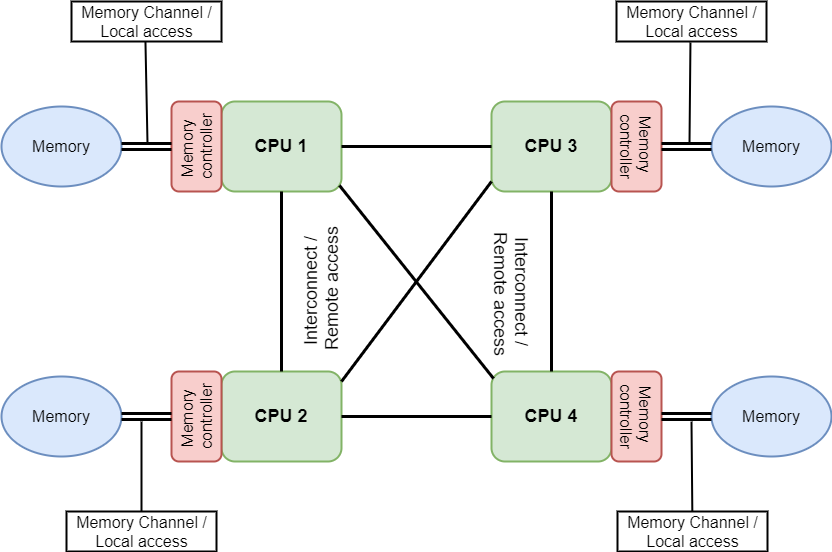
\includegraphics[width=4.0cm]{assets/NUMA.png}

{\tiny From \href{https://docs.lxp.lu/system/images/NUMA.png}{MeluXina}}

\vspace{0.5cm}

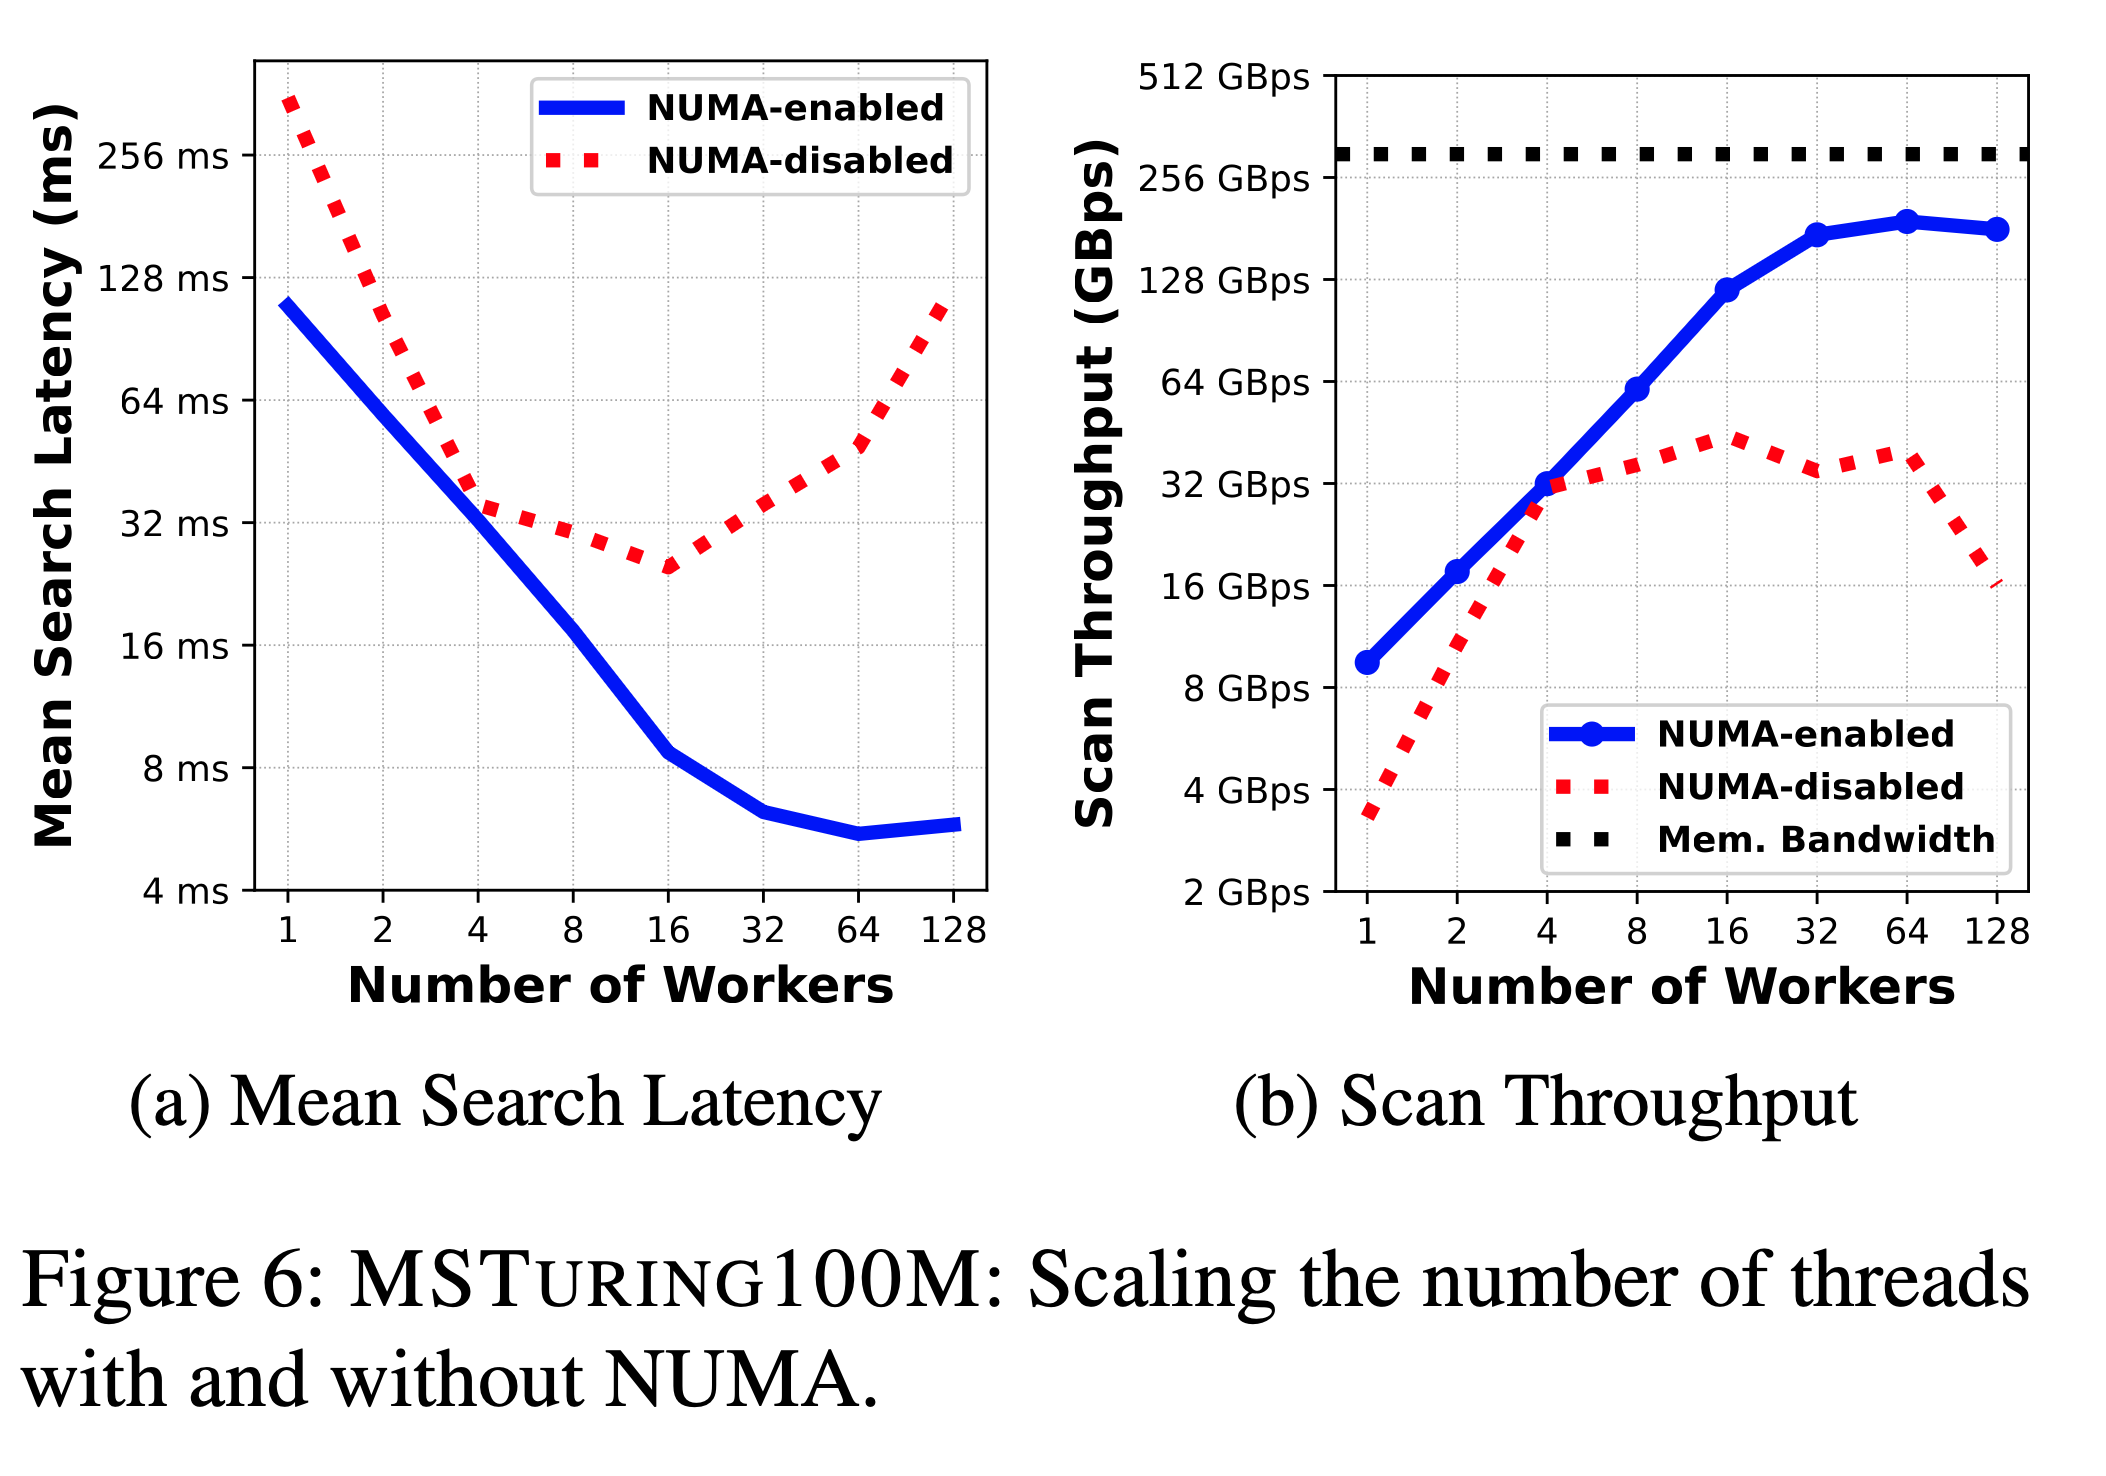
\includegraphics[width=5.5cm]{assets/numa_fig.png}
\end{center}
\end{columns}
\end{frame}
\placelogotrue


\section{Results}

\subsection{Datasets}

%\placelogofalse
\begin{frame}{Wikipedia-12M}
\begin{columns}
\column{0.58\linewidth}
\centering
\begin{outline}
  \1 public dataset and workload trace
\end{outline}

\column{0.38\linewidth}
\begin{center}
\centering
%\shadowimage[width=2.5cm]{example_1.png}

%\includegraphics[width=2.5cm]{example_3.png}
\end{center}
\end{columns}
\end{frame}
%\placelogotrue

%\placelogofalse
\begin{frame}{Wikipedia-12M: Ablation Study}
\begin{columns}
\column{0.48\linewidth}
\centering
\begin{outline}
  \1 APS
  \2 Little impact on latency
  \2 Big impact on Recall
  \1 NUMA Parallelism
  \2 6x speedup
  \1 Maintenence
  \2 Big impact on latency
  \2 Match results from Faiss-IVF
\end{outline}

\column{0.48\linewidth}
\begin{center}
\centering
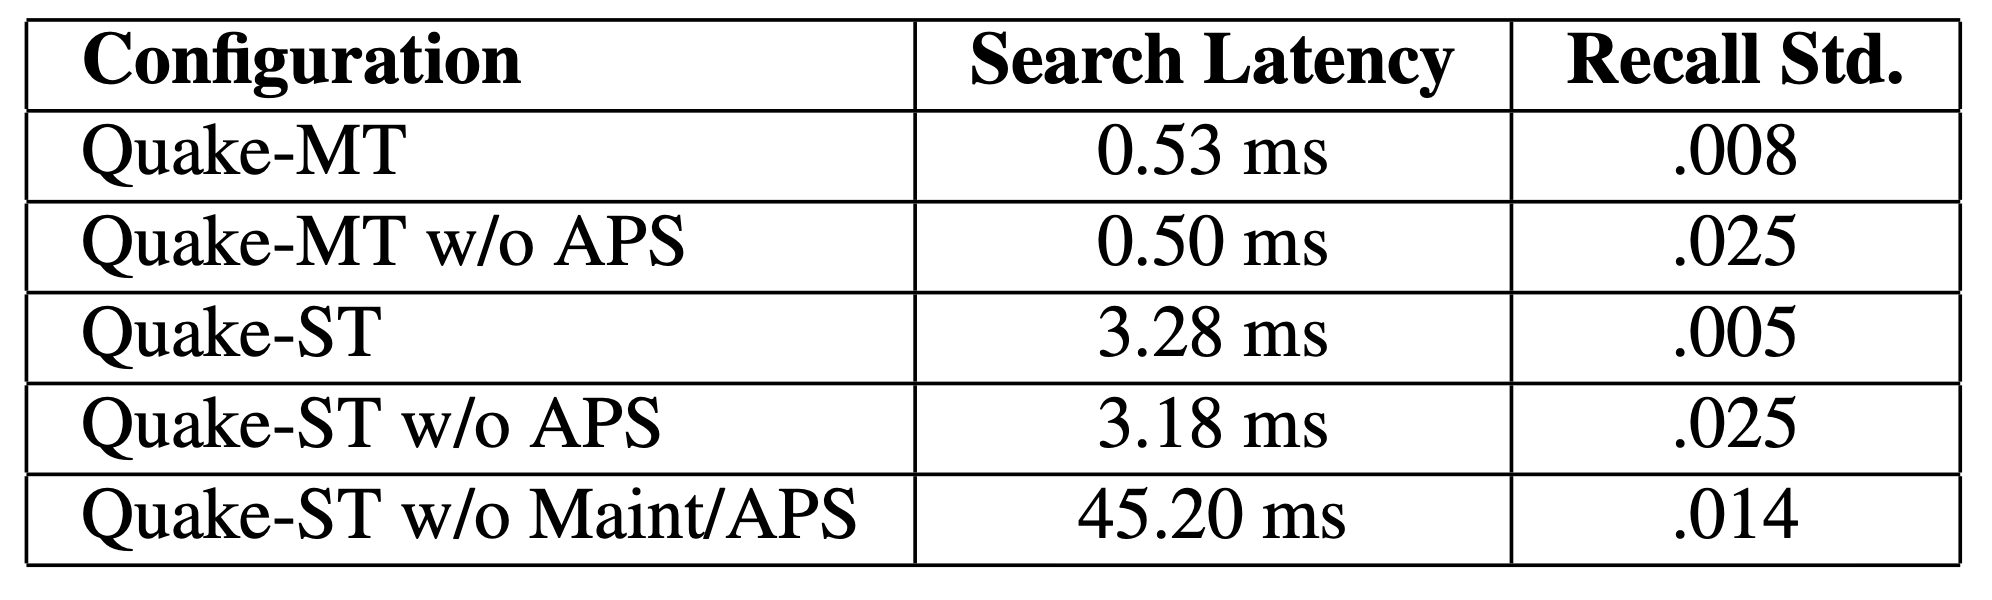
\includegraphics[width=5.5cm]{assets/wiki_ablation.png}
\end{center}
\end{columns}
\end{frame}
%\placelogotrue

%\placelogofalse
\begin{frame}{Other Datasets}
\begin{columns}
\column{0.58\linewidth}
\centering
\begin{outline}
  \1 OpenImages-13M
  \1 MSTuring (10M vector subset)
\end{outline}

\column{0.38\linewidth}
\begin{center}
\centering
%\shadowimage[width=2.5cm]{example_1.png}

%\includegraphics[width=2.5cm]{example_3.png}
\end{center}
\end{columns}
\end{frame}
%\placelogotrue


\begin{frame}{Conclusion}
  \begin{outline}
  \1 Today we've introduced Taichi
  \2 Python based implementation
  \2 Design Goals
  \2 Applications and Research Projects
  \2 Sparse Data Structures
  \1 Questions?
  \end{outline}
\end{frame}


%\begin{frame}[allowframebreaks]{References}
%    \tiny
%    \printbibliography
%\end{frame}

\end{document}


